%%%%%%%%%%%%%%%%%%%%%%%%%%%%%%%%%%%%%%%%%%%%%%%%%%%%%%%%%%%%%%%%%%% 
%                                                                 %
%                            CHAPTER                              %
%                                                                 %
%%%%%%%%%%%%%%%%%%%%%%%%%%%%%%%%%%%%%%%%%%%%%%%%%%%%%%%%%%%%%%%%%%% 

\chapter{Introduction}

    The steel industry is a big industry in the world and provides 2.5 million jobs across Europe according to the European commission. Due to high labour costs in western Europe and more specific in Belgium where they are 40\% above the average of Europe, production and manufacturing costs should decrease to be able to compete with other companies around the world. 
    
For this thesis we focus on metal carving which is done by spinning a spindle over the metal work piece that carves away material. This spindle holds inserts as seen in Figure \ref{fig:intr:inserts} where a top and side view of the insert are provided. A full assemble of the tool and the insert can be found in Figure \ref{fig:gen:insertholder}. The inserts are kept in place with a screw for easy removal and replacement and are made of different compositions of Wolfram carbide. After creation they get a coating on the outer layer to provide extra strength and more capabilities for cutting different materials. 

\begin{figure}[hbtp]
\centering
	\begin{subfigure}{0.45\textwidth}
		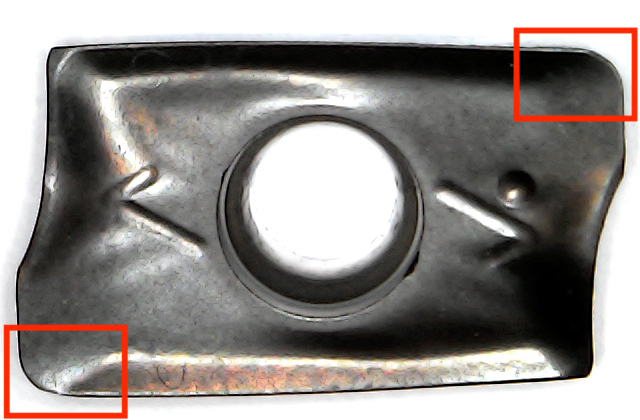
\includegraphics[width=\linewidth]{fig/algemeen/plaatjes/plaatje/top_view_mark.jpg} 
		\caption{Top view}
		\label{fig:gen:insert:top}
	\end{subfigure}
	\hspace*{\fill}
	\begin{subfigure}{0.45\textwidth}
		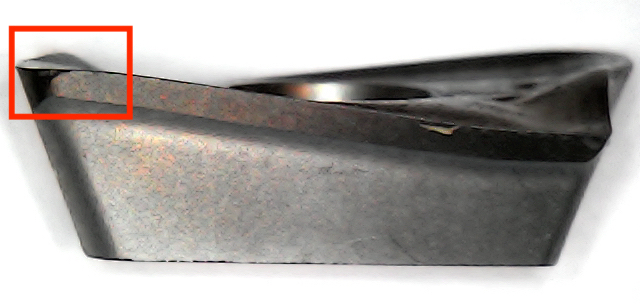
\includegraphics[width=\linewidth]{fig/algemeen/plaatjes/plaatje/side_view_mark.jpg} 
		\caption{Side view}
		\label{fig:intr:insert:side}
	\end{subfigure}
	\caption{Images of the examined carbide tool inserts. The red square marks the area of interest for the wear prediction.}
	\label{fig:intr:inserts}
\end{figure}

\begin{figure}[hbtp]
\centering
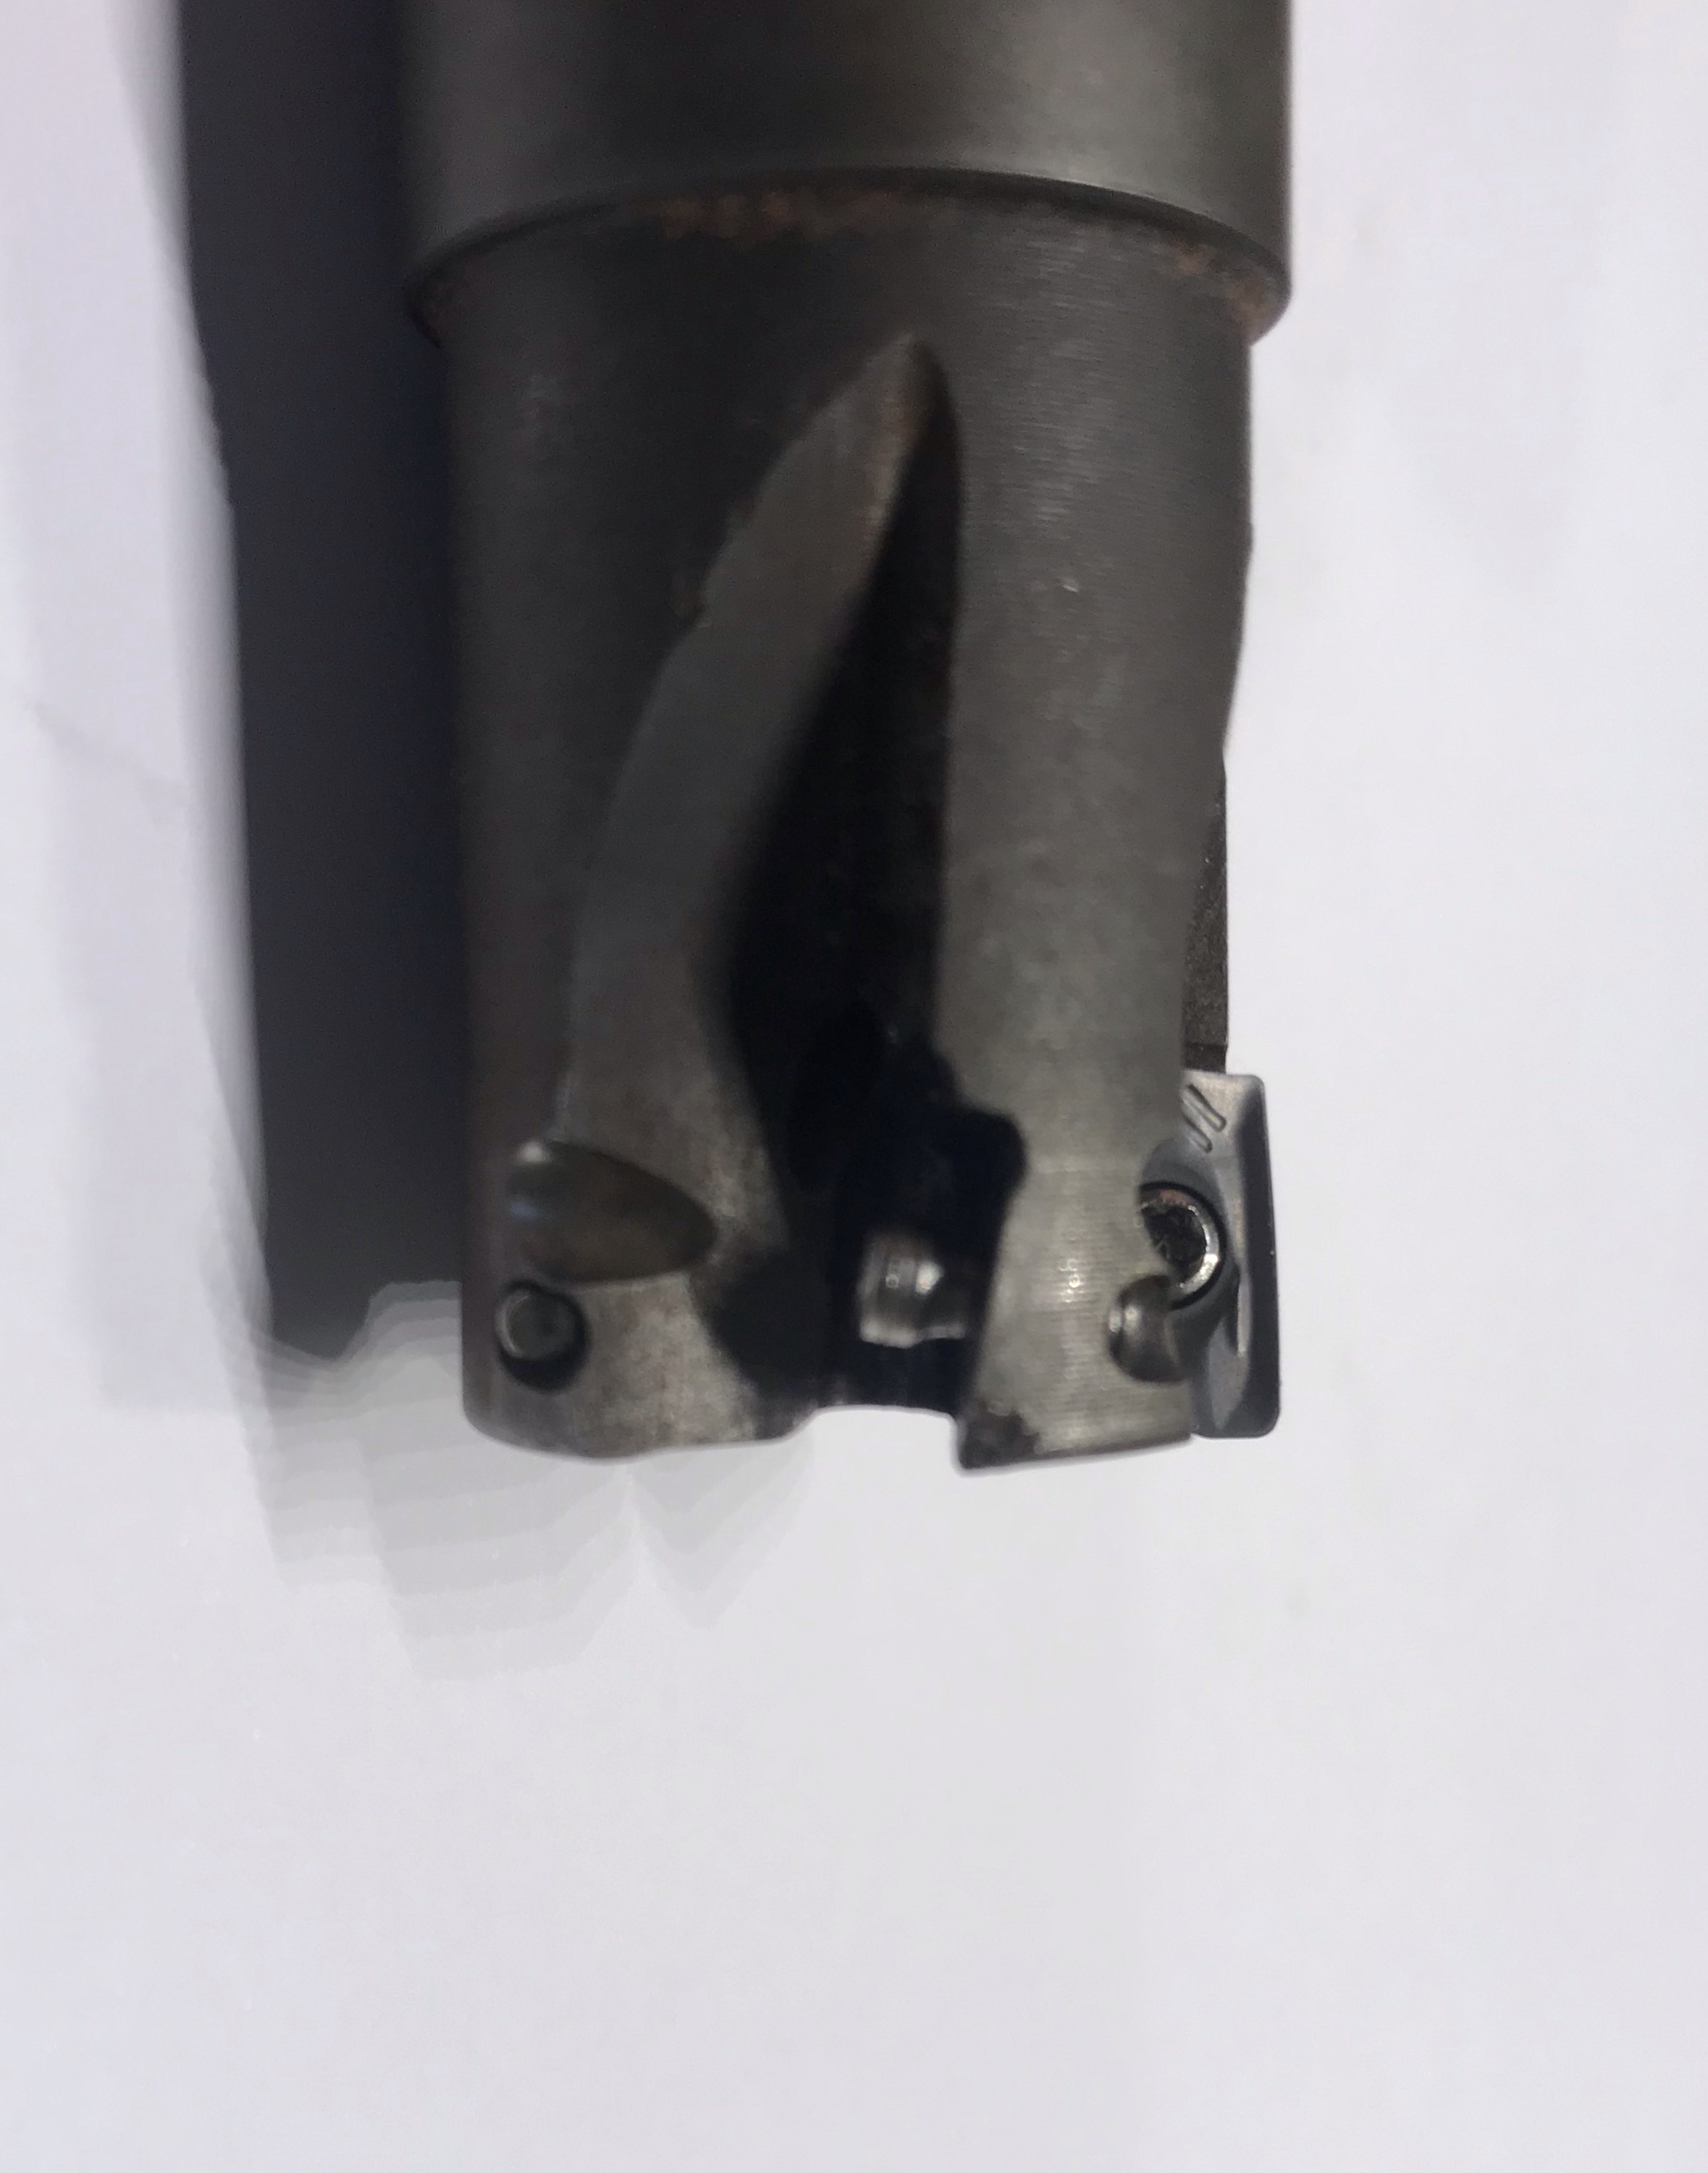
\includegraphics[width=.40\textwidth]{fig/algemeen/plaatjes/houder/rotary_holder.jpeg}
\caption{Milling tool with one insert in place.}
 \label{fig:gen:insertholder}
\end{figure}

The cutting part on the corner of the insert - as marked on Figures \ref{fig:gen:insert:top} and \ref{fig:intr:insert:side} with a red square - will wear when the work piece is carved and will result in a bad finish on the actual product. This can be referred to as surface roughness. To prevent the formation of surface roughness the tool inserts must be replaced before they are worn to much. For this replacement there are two policies used in the industry today:
    \begin{enumerate}
        \item Check the inserts when a work piece is finished.
        \item Replacing all inserts on set time intervals (e.g. every 30 minutes).
    \end{enumerate}
     Although option number one will optimize the lifespan of the inserts, it is very time consuming and labour intensive. Option number two is less labour intensive and thus less time consuming. On the other hand will it produce a lot of waste in those inserts when incorporating safety levels for the wear. 


What does a worn insert look like? This is shown in Figure \ref{fig:intr:insert:wnw} which is a close up from the area marked with a red square from Figure \ref{fig:intr:insert:side}.
Figure \ref{fig:intr:insert:wnw} gives examples of a barely used insert and one of an unusable insert due to the high wear.

\begin{figure}[hbtp]
\centering
	\begin{subfigure}{0.49\textwidth}
		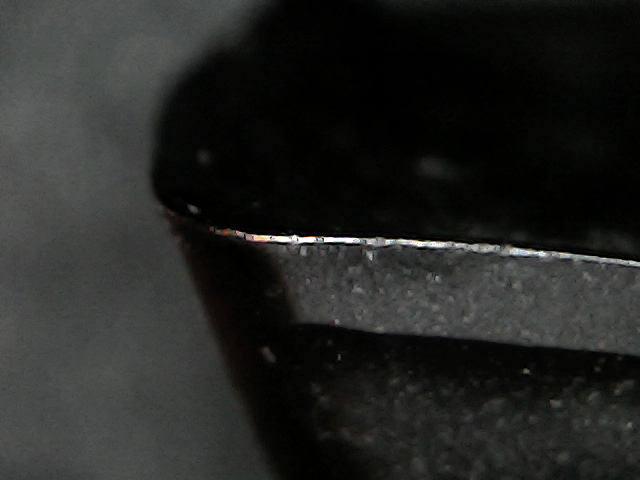
\includegraphics[width=\linewidth]{fig/algemeen/plaatjes/plaatje/n_worn_insert.jpg}
		\caption{Barely used carbide insert.}
	\end{subfigure}
	\hspace*{\fill}
	\begin{subfigure}{0.49\textwidth}
		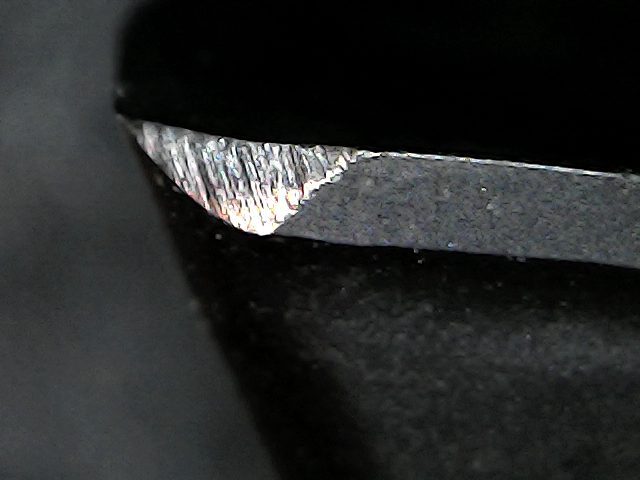
\includegraphics[width=\linewidth]{fig/algemeen/plaatjes/plaatje/worn_insert.jpg} 
		\caption{Worn carbide insert.}
	\end{subfigure}
	\caption{Illustration of a good and a worn insert.}
	\label{fig:intr:insert:wnw}
\end{figure}

     
     The goal for this master thesis is to create a direct measurement method to quantize tool wear on these inserts. From this goal the research questions can be extracted: 
     \begin{itemize}
     	\item "How can tool wear on carbide inserts be quantized by using a direct (vision based) method?"
     	\item "How can a vision set up be implemented in a production line?"
     	\item "What should the vision set up look like?"
     	\item "What computer vision algorithms perform best for this task?"
     \end{itemize}
     	
     	
     For this report however only the foundations are laid where a highly adjustable setup is created as well as some datasets and an algorithm to measure the performance of a specific setup.
     
     
The problem will be split up into two main parts: 
	\begin{itemize}
		\item Creating a camera setup to capture images of the inserts.
		\item Create a vision algorithm to process the images and output the tool wear.
	\end{itemize}
	
We start with a study on the "state of the art" in solving similar problems in chapter \ref{chap:lit}. The construction and implementation of our own method will be discussed in chapter \ref{chap:impl}. Results and datasets will be handled in chapter \ref{chap:results}. And in chapter \ref{chap:conc} we draw conclusions and the research questions are revisited.
	
	%First the state of the art for this problem will be discussed along with some extra literature information on the whole of this problem in chapter \ref{chap:lit}. The implementation will be handled next in chapter \ref{chap:impl} where the process of building a solution is bespoken. The results on the setup, and the generated datasets will be discussed in chapter \ref{chap:res}. After this a conclusion is written in chapter \ref{chap:conc} and the research questions are revisited.